\documentclass[titlepage]{article}
\usepackage[utf8]{inputenc}
\usepackage[spanish,activeacute]{babel}
\usepackage{graphicx}
\usepackage{amsmath}   
\usepackage{tikz}
\graphicspath{{Imagenes/}}

\begin{document}
   
    \begin{titlepage}
    
        \centering
        
\includegraphics[width=0.25\textwidth]{EmblemaUnicauca}\par\vspace{1cm}
        \textbf{\LARGE UNIVERSIDAD DEL CAUCA}\par\vspace{1cm}
        \textbf{\Large Facultad de Ingeniería Civil}\par\vspace{1cm}
        \textbf{\Large SISTEMAS DE ECUACIONES DIFERENCIALES LINEALES DE PRIMER ORDEN}\par\vspace{1cm} 
        \textbf{\Large Presentado a:}\par\vspace{0.5cm}
        \large Prof. Jonathan Collazos Ramirez\par\vspace{1cm}
        \textbf{\Large Presentado por:}\par\vspace{0.5cm}
        \large Cristhian Andres Medina Ordoñez\par\vspace{1cm}
        \textbf{\Large Curso:}\par\vspace{0.5cm}
        \large Ecuaciones Diferenciales Ordinarias \par\vspace{1cm}
        Documento realizado en \LaTeX
        \vfill
        \textbf{\large Popayán - Cauca}\par
        \textbf{\large Agosto 2022} 
        
    \end{titlepage}
    
    \tableofcontents
    
    \vfill
    
    \section{Introducción}
    
        Las ecuaciones diferenciales de manera general son igualdades que relacionan funciones con sus derivadas (o variaciones de ciertas condiciones respecto de parametros que se quieran estudiar). Esto se realiza analizando las condiciones del fenómeno o situación especifica que se quiera observar; se analiza la variación de las condiciones que se quiera y esto es posible lograrlo en muchos casos, con ayuda de la física y de las ecuaciones diferenciales. La física aporta principios del comportamiento del entorno y de los fenomenos que suceden en el mismo. \par\vspace{0.4cm}
        El curso de ecuaciones diferenciales permite hacer frente a los problemas que se presentan donde existen relaciones entre un estado inicial y un siguiente estado de acuerdo a la variación de cada parámetro respecto de una o más variables (derivadas ordinarias y/o parciales) a analizar. Posteriormente, con ayuda de metodos desarrollados a lo largo de las décadas y que dependen del tipo de ecuación que se tenga, se pueden resolver dichas ecuaciones. Cabe resaltar, que para el desarrollo correcto de la solución de una ecuación diferencial, es necesario conocer muy bien las ecuaciones diferenciales (su tipo, orden, grado, estructura, etc), ya que de esto depende mayormente el método de solución que se debería utilizar y su correcta solución.\par\vspace{0.4cm}
        Ahora bien, ademas de conocer la solución de ecuaciones diferenciales mediante distintos métodos para dar solución a sistemas de ecuaciones diferenciales, se hace necesario el conocimiento y dominio de las herramientas otorgadas en el curso de Algebra Lineal, ya que el manejo mas cómodo para un sistema de ecuaciones ya sea diferencial o no, es el manejo matricial aprendido en dicho curso. Y ademas, al haber sistemas de ecuaciones, se presentarán matrices con las cuales será necesario trabajar.\par\vspace{0.4cm}
        Este documento se enfocará únicamente en los \textbf{sistemas de ecuaciones diferenciales lineales de primer orden.} \par\vspace{5cm}
        \vfill
    
    \section{Conceptos y teoría básica}
        
        

        \subsection{Definición de Sistema de Ecuaciones Diferenciales Lineales de Primer Orden}\par
        
        De acuerdo con Boyce y Diprima: Existen muchos problemas físicos que comprenden varios elementos separados entre si vinculados de alguna manera y en muchos casos, el problema matemático correspondiente consta de un sistema de una o mas ecuaciones diferenciales, que siempre es posible escribir como ecuaciones de primer orden.\cite{Boyce2003}\par\vspace{0.4cm}
        Teniendo en cuenta su importancia, es necesario reconocer el orden de una ecuacion diferencial, sus coeficientes y la estructura general de la ecuación. Una ecuación diferencial de primer orden, como su nombre lo dice, posee derivadas de orden uno y no mayor;ademas la linealidad de la ecuación se verifica con el exponente que posean las primeras derivadas de la función (o variable dependiente de la ecuación) o dicha función, y tambien con las funciones que acompañan a las derivadas o a la función; ya que estas no pueden incluir en su estructura a la variable dependiente. Es decir, segun Zill se puede definir un sistema de ecuaciones diferenciales lineales de primer orden, de la siguiente manera: \par\vspace{0.4cm}
        
        Los sistemas de ecuaciones diferenciales lineales de primer orden son casos especiales de los sistemas de ecuaciones diferenciales, los cuales tienen la siguiente forma (Forma normal):\par\vspace{0.4cm}
        
        \begin{equation*}
            \frac{dX_1}{dt}  = g_1(t,X_1,X_2,...,X_n)
        \end{equation*}
        \begin{equation*}   
            \frac{dX_2}{dt}  = g_2(t,X_1,X_2,...,X_n)
        \end{equation*}
       
        \begin{equation*}   
            \frac{dX_n}{dt} = g_n(t,X_1,X_2,...,X_n)
        \end{equation*}\vspace{0.2cm}
            
            
        Este es el conocido \textbf{sistema de ecuaciones diferenciales de primer orden.}\cite{Zill2002}\par\vspace{0.5cm}
        
        \textbf{\large SISTEMA LINEAL}\par\vspace{0.2cm}
        
        Ahora, si se considera que las funciones g, son lineales en las variables dependientes $X_1,X_2,...,X_n$, entonces el sistema de primer orden se vuelve un \textbf{sistema de ecuaciones lineales de primer orden:}\par
        
    
        
        \begin{equation*}
            \frac{dX_1}{dt} = a_{11}(t)X_1 + a_{12}(t)X_2 + ... + a_{1n}(t)X_n + f_1(t)
        \end{equation*}
        \begin{equation*}   
           \frac{dX_2}{dt}  = a_{21}(t)X_1 + a_{22}(t)X_2 + ... + a_{2n}(t)X_n + f_2(t)
        \end{equation*}
        
        \begin{equation*}   
            \frac{dX_n}{dt} = a_{n1}(t)X_1 + a_{n2}(t)X_2 + ... + a_{nn}(t)X_n + f_n(t)
        \end{equation*}\vspace{0.2cm}
        
        Se supone que los coeficientes $a_{nn}(t)$ y las funciones f son continuas en un intervalo I en común. Ademas, si las funciones de la forma $f_n(t)$ son iguales a cero, entonces el sistema se llama \textbf{Sistema homogéneo}; en caso contrario será un \textbf{Sistema NO homogéneo}.\cite{Zill2002}
            
        \subsection{Teoría básica de los sistemas lineales de primer orden}\par\vspace{0.3cm}
        
        Un conjunto de funciónes de la forma $y = f(x)$  son solución de la ecuación (organizadas matricialmente forman el vector solución), si se cumple que para cada primera derivada de $X_i$ y la funcion $X_i$, al reemplazarla en las ecuaciones correspondientes, se llega a una identidad en cada ecuación del sistema, donde cada $X_i$ y sus primeras derivadas lo satisfacen.\par\vspace{0.4cm}
        Tambien se asume que si las funciones que dependen unicamente de la variable independiente de la forma f(t) son \textbf{cero}, el sistema se convierte en homogeneo. Ademas se hace uso de la escritura en forma matricial para trabajar mas comodamente y evitar perder tiempo en la escritura de largas ecuaciones diferenciales, quedando así:
        
        \begin{equation}
            \Vec{X'} = A(t)\Vec{X}
            \label{1}
        \end{equation}
        
        Entiendase que en (\ref{1}), $\Vec{X'}$ se refiere al vector columna compuesto por las primeras derivadas de las funciones soluciones $X_n$, A(t) se refiere a la matriz de coeficientes de cada una de las componentes de las ecuaciones y $\vec{X}$ se refiere al vector solución, el cual contiene las funciones que satisfacen el sistema (estas funciones son desconocidas inicialmente).\cite{Kreyszing2003} \par\vspace{0.4cm}
        
        Es decir, \par\vspace{0.4cm}
        
        \begin{equation*}
            \Vec{X'} = 
            \begin{pmatrix}
                X'_1 \\ 
                X'_2 \\ 
                X'_n 
            \end{pmatrix}
        \end{equation*} \par\vspace{0.4cm}
        
        \begin{equation*}
            A(t) = 
            \begin{pmatrix}
                a_{11} & a_{12} & a_{1n} \\ 
                a_{21} & a_{22} & a_{2n} \\ 
                a_{n1} & a_{n2} & a_{nn} 
            \end{pmatrix}
        \end{equation*} \par\vspace{0.4cm}
        
        \begin{equation*}
            \Vec{X} = 
            \begin{pmatrix}
                X_1 \\ 
                X_2 \\ 
                X_n 
            \end{pmatrix}
        \end{equation*} \par\vspace{0.4cm}
        
        
        \subsubsection{Problemas con Valores Iniciales}
                
            Sea $t_0$ que denota un punto en el intervalo I y se tiene que, 
        
        \begin{equation*}
            \Vec{X}(t_0) =
            \begin{pmatrix}
                X_1(t_0) \\
                X_2(t_0) \\
                X_n (t_0)
            \end{pmatrix}
        \end{equation*}   
        y    
        \begin{equation*}
            \Vec{X_0} =
            \begin{pmatrix}
                r_1 \\
                r_2 \\
                r_n
            \end{pmatrix}
        \end{equation*}   
        
        donde las $r_i$, $i = 1,2,...,n$ son las constantes dadas. Entonces el problema,\vspace{0.3cm}
            Resolver:
            \begin{equation*}
                \Vec{X'} = A(t)\Vec{X} + \Vec{F}(t)
            \end{equation*}
            Sujeto a: 
            \begin{equation*}
                \Vec{X}(t_0) = \Vec{X_0}
            \end{equation*}
            Es un problema con \textbf{ valores iniciales en el intervalo I.}\cite{Zill2002a}
        \subsubsection{Teorema de Existencia de Solución Unica}\par\vspace{0.3cm}
            
            Se tiene que, \par\vspace{0.1cm}
                \begin{equation*}
                    \vec{X}' = A(t)\vec{X} + \vec{F}(t), 
                \end{equation*}
                
            y sean los elementos de las matrices \textbf{A(t) y $\vec{F}$(t)} funciones continuas en un intervalo común I que contiene al punto $t_0$. Entonces existe una solución única del sistema del que se cuenta con valores iniciales en el intervalo.\cite{Zill2002a}     
            
        \subsection{Teoría correspondiente a Sistemas de Ecuaciones Diferenciales Lineales Homogéneos}\par\vspace{0.3cm} 
        
            \subsubsection{Definición de Vector Solución}
            Un vector solución en un intervalo I, es un vector columna de la forma,\par 
                
            
                    
                    \begin{equation*}
                        \vec{X} =
                        \begin{pmatrix}
                            
                            X_1(t) \\
                            X_2(t) \\
                            \vdots \\
                            X_n(t)
                        
                        \end{pmatrix} 
                    \end{equation*}
                           
            Por ejemplo, si se quisiera comprobar que un par de vectores $\vec{X_1}$ y $\vec{X_2}$ son solución de un sistema homogéneo, siendo dichos vectores:
        
            \begin{equation*}
                \vec{X_1} = 
                \begin{pmatrix}
                    e^{-2t} \\
                    -e^{-2t}
                \end{pmatrix}
            \end{equation*}
            y,
            \begin{equation*}
                \vec{X_2} =
                \begin{pmatrix}
                    3e^{6t} \\
                    5e^{6t}
                \end{pmatrix}
            \end{equation*}\vspace{0.1cm}
            Y el sistema es el siguiente:
            \begin{equation*}
                X' = 
                \begin{pmatrix}
                    1 & 3 \\
                    5 & 3
                \end{pmatrix}   
                X
            \end{equation*}
            
            Entonces lo que se debe hacer es evaluar dichas soluciones en el sistema, primeramente obteniendo las derivadas de $\vec{X_1}$ y $\vec{X_2}$, 
            
                \begin{equation*}
                    \vec{X_1'} = 
                    \begin{pmatrix}
                        -2e^{-2t}\\
                        2e^{-2t}
                    \end{pmatrix}
                \end{equation*}
            y,
                 \begin{equation*}
                    \vec{X_2'} = 
                    \begin{pmatrix}
                        18e^{6t}\\
                        30e^{6t}
                    \end{pmatrix}
                \end{equation*} 
            Ahora, ya se puede evaluar cada una de los vectores solución en el sistema y se debe llegar a una identidad.\par\vspace{0.2cm}
            
            Para $X_1$:    
                \begin{equation*}
                    \begin{pmatrix}
                        -2e^{-2t}\\
                        2e^{-2t}
                    \end{pmatrix} =
                    \begin{pmatrix}
                        1 & 3 \\
                        5 & 3
                    \end{pmatrix}   
                    \begin{pmatrix}
                        e^{-2t} \\
                        -e^{-2t}
                    \end{pmatrix}
                \end{equation*}
                
            Para $X_2$:
                
                \begin{equation*}
                    \begin{pmatrix}
                        18e^{6t}\\
                        30e^{6t}
                    \end{pmatrix} =
                    \begin{pmatrix}
                        1 & 3 \\
                        5 & 3
                    \end{pmatrix}   
                    \begin{pmatrix}
                        3e^{6t} \\
                        5e^{6t}
                    \end{pmatrix}
                \end{equation*}
                
            Si se resuelve la multiplicación de la matriz por el vector columna $X_i$, se debe llegar a una igualdad verdadera:\par\vspace{0.2cm}
            
            Para $X_1$ se tiene,
            
                \begin{equation*}
                    \begin{pmatrix}
                        -2e^{-2t}\\
                        2e^{-2t}
                    \end{pmatrix}=
                    \begin{pmatrix}
                        e^{-2t}-3e^{-2t}\\
                        5e^{-2t}-3e^{-2t}
                    \end{pmatrix}
                \end{equation*}   
                
            Para $X_2$ se tiene,
            
                \begin{equation*}
                    \begin{pmatrix}
                        18e^{6t}\\
                        30e^{6t}
                    \end{pmatrix}=
                    \begin{pmatrix}
                        3e^{6t} + 15e^{6t}\\
                        15e^{6t} + 15e^{6t}
                    \end{pmatrix}
                \end{equation*}\vspace{0.3cm}   
           Por tanto se observa que se llega a una \textbf{identidad}, y por eso se dice que los vectores $\vec{X_1}$ y $\vec{X_2}$ son \textbf{Vectores Solución del sistema.}
           
        \subsubsection{Principio de Superposición}
            
            Este teorema indica que si se tienen $X_1,X_2,...,X_n$ funciones vectoriales y siendo éstas, solución de un sistema de ecuaciones diferenciales lineal de primer orden homogéneo entonces cualquier combinación lineal de la forma,
                \begin{equation}
                    \vec{X} = c_1\vec{X_1} + c_2\vec{X_2} + ... + c_n\vec{X_n}
                \end{equation}
            
            Siendo $\vec{X}$ y $\vec{X_n}$ en todos los casos vectores solución del sistema, es \textbf{tambien solución del sistema.}\cite{Boyce2003a}\par\vspace{0.2cm}
            
            Por ejemplo, se puede verificar que un par de vectores $\vec{X_1}$ y $\vec{X_2}$ son solución de un sistema, mediante el uso del teorema de superposición, de la siguiente manera:\par
            Si se tiene que,
                \begin{equation*}
                    \vec{X_1} =
                    \begin{pmatrix}
                        3e^{2t}\\
                        2e^{2t}
                    \end{pmatrix}
                \end{equation*}
           y,
                 \begin{equation*}
                    \vec{X_2} =
                    \begin{pmatrix}
                        e^{-5t}\\
                        3e^{-5t}
                    \end{pmatrix}
                \end{equation*}
                
            y ademas se tiene el sistema:
            
                \begin{equation*}
                    \vec{X'} = 
                    \begin{pmatrix}
                        4 & -3 \\
                        6 & -7
                    \end{pmatrix}   
                    \vec{X}
                \end{equation*}
                
            Lo que se debe hacer es buscar una combinación lineal de la forma:
            
                \begin{equation*}
                    \vec{X} = c_1\vec{X_1} + c_2\vec{X_2} 
                \end{equation*}  
                
            es decir,
                
                \begin{equation*}
                    \vec{X} = c_1
                    \begin{pmatrix}
                        3e^{2t}  \\
                        2e^{2t} 
                    \end{pmatrix}   
                    + c_2
                    \begin{pmatrix}
                        e^{-5t}  \\
                        3e^{-5t} 
                    \end{pmatrix}   
                \end{equation*}
                
            A continuacion se derivará $\vec{X}$ quedando,
                
                \begin{equation*}
                    \vec{X'} = 
                    \begin{pmatrix}
                        6c_1e^{2t}  \\
                        4c_1e^{2t} 
                    \end{pmatrix} +  
                    \begin{pmatrix}
                        -5c_2e^{-5t}  \\
                        -15c_2e^{-5t} 
                    \end{pmatrix}   
                \end{equation*}        
            Como ya tenemos el valor de $\vec{X'}$ ahora, obtengamos $A\vec{X}$, esto es,
                
                \begin{equation*}
                    A\vec{X} = 
                    \begin{pmatrix}
                        4 & -3 \\
                        6 & -7
                    \end{pmatrix}   
                    \begin{pmatrix}
                        3c_1e^{2t}+c_2e^{-5t} \\
                        2c_1e^{2t}+3c_2e^{-5t}
                    \end{pmatrix}
                \end{equation*}    
                 
                \begin{equation*}
                    = 
                    \begin{pmatrix}                                                            12c_1e^{2t}+4c_2e^{-5t}-6c_1e^{2t}-9c_2e^{-5t} \\
                        18c_1e^{2t}+6c_2e^{-5t}-14c_1e^{2t}-21c_2e^{-5t}
                    \end{pmatrix}
                \end{equation*}
                Operando se tiene,
                
                    \begin{equation*}
                    A\vec{X}= 
                    \begin{pmatrix}                                                            6c_1e^{2t}-5c_2e^{-5t} \\
                        4c_1e^{2t}-15c_2e^{-5t}
                    \end{pmatrix}
                \end{equation*}
                
                Podemos observar que $A\vec{X}=\vec{X'}$, por tanto el principio de superposición se cumple.
                
                
        \subsubsection{Dependencia o Independencia Lineal} 
            Si se tiene un conjunto de soluciones de un sistema lineal homogéneo de la forma, \par\vspace{0.1cm}
            \begin{center}
                $\vec{X_1}$,$\vec{X_2}$,...,$\vec{X_n}$
            \end{center} 
            y si por medio de una combinación lineal de dichos vectores, utilizando unas constantes $c_1$,$c_2$,...,$c_n$ se puede comprobar que:
            
                \begin{equation*}
                    c_1\vec{X_1} + c_2\vec{X_2} + ... + c_n\vec{X_n} = \vec{0}       
                \end{equation*}\vspace{0.2cm}
            entonces, se dice que el conjunto de soluciones es \textbf{linealmente dependiente}, en el intervalo I. En caso contrario, es decir cuando no se pueda encontrar dichos valores, se dirá entonces que el conjunto de soluciones es \textbf{linealmente independiente.}\cite{Zill2002a}  
            
        \subsubsection{Criterio para las soluciones linealmente independientes}
        
            Si se tienen los vectores solución del sistema lineal homogéneo denotados $X_1,X_2,...,X_n$ y se obtiene el determinante de la matriz obtenida de dichos vectores solución, mediante el Wronskiano de la matriz. Si se cumple que,
            
                \begin{equation*}
                    \centering
                    W(\vec{X_1},\vec{X_2},...,\vec{X_n}) = 
                    \begin{vmatrix}
                       
                        X_{11} & X_{12} &...& X_{1n} \\
                        
                        X_{21} & X_{22} &...& X_{2n} \\
                        
                        X_{n1} & X_{n2} &...& X_{nn}
                        
                    \end{vmatrix}
                    \neq 0
                \end{equation*}\vspace{0.2cm}
                
            entonces el conjunto es \textbf{linealmente independiente.} \cite{Zill2002a}
            
        \subsubsection{Definicion de conjunto fundamental de Soluciones}   
        
            Si se tiene un conjunto de soluciones de tipo $\vec{X_1},\vec{X_2},...,\vec{X_n}$ que son solución de un sistema lineal homogéneo y ademas este conjunto es \textbf{linealmente independiente} $(W \neq 0)$, entonces este conjunto se denomina \textbf{Conjunto fundamental de soluciones en el intervalo I.} \cite{Zill2002a}
          
        \subsubsection{Existencia de un conjunto fundamental}  
            Existe un conjunto fundamental de soluciones para un sistema lineal homogéneo de la forma expuesta en  (\ref{1}), en el intervalo I.
            
        \subsubsection{Solución General de Sistemas Homogéneos} 
            Si se tiene un conjunto fundamental de soluciones de la forma $\vec{X_1},\vec{X_2},...,\vec{X_n}$ del sistema lineal homogeneo de la forma expuesta en  (\ref{1}), entonces la \textbf{solucion general del sistema} en el intervalo I es,
            
                \begin{equation*}
                    \vec{X} = c_1\vec{X_1} + c_2\vec{X_2} +...+ c_n\vec{X_n}
                \end{equation*}
            Donde $\vec{X},\vec{X_1},\vec{X_2},...,\vec{X_n}$ son funciones vectoriales y $c_1,c_2,...,c_n$ son constantes arbitrarias.
            
    \subsection{Sistemas Lineales homogéneos de Coeficientes constantes}
            
        Es un sistema lineal de la forma ya conocida $\vec{X'} = A\vec{X}$ y se denomina de coeficientes constantes debido a que la matriz A es de valores constantes.
        Para la solución de los sistemas lineales homogéneos de primer orden y con coeficientes constantes, se utiliza el metodo de valores y vectores propios (eigen valores y eigen vectores) despejando los valores de $\lambda$ de resolver el Wronskiano $det(A-\lambda I) = 0 $, donde I es la matriz identidad de diagonal con valores de 1 y las demas casillas 0.\par\vspace{0.2cm} 
        Pero estos valores propios pueden ser diferentes entre sí, ser iguales entre sí o o tener valores complejos. 
            
            \subsubsection{Valores propios reales y distintos}
                Cuando la matriz A, cuadrada, tiene $n$ valores propios reales y distintos de la forma $\lambda_1,\lambda_2,...,\lambda_n$, siempre se pueden encontrar un conjunto de $n$ vectores propios $\vec{K_1},\vec{K_2},...,\vec{K_n}$ y tambien se cumple que, 
                \begin{equation*}
                    \vec{X_1} = \vec{K_1}e^{\lambda_1t}
                \end{equation*}
                \begin{equation*}
                    \vec{X_2} = \vec{K_2}e^{\lambda_2t}
                \end{equation*}
            
                \begin{equation*}
                    \vec{X_n} = \vec{K_n}e^{\lambda_nt}
                \end{equation*}
                Es un conjunto fundamental de soluciones de (\ref{1}) en el intervalo ($-\infty,\infty$).\vspace{0.1cm}
                
          Por ejemplo, si se quisiera resolver el sistema:
          
          		\begin{equation*}
          		      \frac{dX_1}{dt} = 2X_1 + 3X_2 
          		          		          										\end{equation*}
          		\begin{equation*}
          		      \frac{dX_2}{dt} = 2X_1 + X_2
      			\end{equation*}
      			
      		Primeramente deberiamos escribirlo en forma matricial de la siguiente manera:
      		
      		\begin{equation*}
      			\vec{X'} =
      			\begin{pmatrix}
      				2 & 3 \\
      				2 & 1
      			\end{pmatrix}
      				\vec{X}
      		\end{equation*}
      		
      	Ademas, asumimos que la forma de la solución es:
      	
      		\begin{equation*}
      			\vec{X} = \vec{K}e^{\lambda t}
      		\end{equation*}
      		
       Si derivamos la expresión anterior tenemos:
       
       		\begin{equation*}
      			\vec{X'} = \lambda \vec{K}e^{\lambda t}
      		\end{equation*}
      	
       Ahora podemos reemplazar $\vec{X}$ y $\vec{X'}$ en la expresión matricial del sistema y esto queda:
       
       		\begin{equation*}
       			\begin{pmatrix}
       				K_1 \\
       				K_2
       			\end{pmatrix}
       			\lambda e^{\lambda t} =
       			\begin{pmatrix}
       				2 & 3 \\
       				2 & 1 
       			\end{pmatrix}
       			\begin{pmatrix}
       				X_1 \\
       				X_2
       			\end{pmatrix}
       			e^{\lambda t}
       		\end{equation*}
       	
       	Si desarrollamos las operaciones tenemos:
       		
       		\begin{equation*}
       			\begin{pmatrix}
       				K_1\lambda e^{\lambda t}\\
       				K_2\lambda e^{\lambda t}
       			\end{pmatrix}
      			=
      			\begin{pmatrix}
      				2K_1e^{\lambda t} + 3K_2e^{\lambda t}\\
      				2K_1e^{\lambda t} + K_2e^{\lambda t}
      			\end{pmatrix}
      		\end{equation*}
      	 Tomando las ecuaciones resultantes de lo anterior se tiene,
      	 
      	 \begin{equation*}
      	 	K_1\lambda e^{\lambda t} = 2K_1e^{\lambda t} + 3K_2e^{\lambda t}
      	 \end{equation*}
      	 	
      	 \begin{equation*}
      	 	K_2\lambda e^{\lambda t} = 2K_1e^{\lambda t} + K_2e^{\lambda t}
      	 \end{equation*}
      	 
      	 Si dividimos las ecuaciones anteriores entre el termino $e^{\lambda t}$ se tiene:
      	 
      	 \begin{equation*}
      	 	K_1\lambda = 2K_1 + 3K_2
      	 \end{equation*}
      	 	
      	 \begin{equation*}
      	 	K_2\lambda  = 2K_1 + K_2
      	 \end{equation*}
      	 
      	 Ahora dejamos las ecuaciones igualadas a cero pasando los terminos de la izquierda a la derecha restando, entonces queda:
      	 
      	 \begin{equation*}
      	 	2K_1 - K_1\lambda + 3K_2 = 0
      	 \end{equation*}
      	 	
      	 \begin{equation*}
      	 	2K_1 + K_2 - K_2\lambda  = 0
      	 \end{equation*}
      	
      	Obteniendo factor común se tiene:
      	
      	 	\begin{equation}
      	 		(2 - \lambda)K_1 + 3K_2 = 0
      	 		\label{3}
      	 	\end{equation}
      	 	
      	 \begin{equation}
      	 	2K_1 + (1 - \lambda)K_2  = 0
      	 	\label{4}
      	 \end{equation}	
      	 
      	 Ahora obtendremos el determinante de la matriz asociada al sistema anterior, es decir:
      	 
      	 \begin{equation*}
      	 	\begin{vmatrix}
      	 		2 - \lambda & 3\\
      	 		2 & 1 - \lambda
      	 	\end{vmatrix}
      	 	= 0
      	  \end{equation*}
      	  
      	  De lo cual se obtiene:
      	  
      	  \begin{equation*}      	  
      	  	2 - 2\lambda - \lambda + \lambda^2 - 6 = 0 	  	
      	  \end{equation*}
      	  
      	  Ordenando y simplificando:
      	  
      	  \begin{equation*}      	  
      	  	\lambda^2 - 3\lambda - 4 = 0 	  	
      	  \end{equation*}
      	  
      	  La ecuación anterior es llamada la \textbf{Ecuación caracteristica de la matriz A.}
      	  
      	  Si se resuelve la ecuación caracteristica, entonces se obtiene los valores propios de A:
      	  
      	  \begin{equation*}
      	  	 \lambda_1 = 4
      	  \end{equation*}	
      	  \begin{equation*}
      	  	 \lambda_1 = -1
      	  \end{equation*}
      	  
      Con estos valores propios se puede determinar los vectores propios. Primeramente se evaluan los valores propios en el sistema de ecuaciones de (\ref{3}) y (\ref{4}) y se tiene:\par\vspace{0.2cm}
      
      	Para $\lambda_1 = 4 $ :
      	
      	\begin{equation*}
      			-2K_1 + 3K_2 = 0
      	\end{equation*}
      	\begin{equation*}
      			2K_1 - 3K_2 = 0
      	\end{equation*}
      	
      	Si dejamos a una variable en terminos de la otra, ya se puede contruir el primer vector propio:
      	
      	\begin{equation*}
      		K_2 = \frac{2}{3}K_1
      	\end{equation*}
      	
      	El vector propio $\vec{K_1}$ queda de la siguiente forma asignandole un valor de 3 a $K_1$:
      	
      		\begin{equation*}
      			\vec{K_1} = 
      			\begin{pmatrix}
      				3\\
      				2	
      			\end{pmatrix}
      		\end{equation*}
      	
      	Realizando exactamente el mismo proceso anterior pero para $\lambda_2 = -1$ y resolviendo el sistema queda:
      	
      		\begin{equation*}
      			K_1 = - K_2
      		\end{equation*}
      	
      	Y tomando valor para $K_2 = 1$
      		
      		\begin{equation*}
      			\vec{K_2} = 
      			\begin{pmatrix}
      				- 1\\
      				1	
      			\end{pmatrix}
      		\end{equation*}
      	
      	Entonces la solución del sistema homogeneo de ecuaciones diferenciales lineales queda:
      	
      	\begin{equation*}
      		\vec{X} = c_1
      		\begin{pmatrix}
      			3\\
      			2	
      		\end{pmatrix}
      		e^{4t} + c_2 
      		\begin{pmatrix}
      			- 1\\
      			1
      		\end{pmatrix}
      		e^{- t}
      	\end{equation*}
      
      		
      			
      		
      	
      	
      
      	  
      	 		
            \subsubsection{Valores propios reales y repetidos}
            
                No necesariamente, los valores propios de una matriz son diferentes entre si, en ocasiones se da que los valores caracteristicos de una matriz son iguales.\par\vspace{0.1cm}
                
                \textbf{Caso 1}. Si sólo hay un eigenvector propio que corresponde al eingenvalor de multiplicidad m, entonces siempre se pueden encontrar m soluciones linealmente independientes y se pueden expresar como combinación lineal de la forma conocida, \cite{Zill2002b}
                    
                    \begin{center}
                        $c_1K_1e^{\lambda_1t}$ + $c_2K_2e^{\lambda_1t}$ + ... + $c_mK_me^{\lambda_1t}$
                    \end{center}
                    
                \textbf{Caso 2}.  Si un valor de $\lambda$ obtenido se repite, entonces se dice que ese $\lambda$ es de multiplicidad m, siendo m el numero de veces que se repite dicha raiz.\par
                Si se tiene un solo valor propio $\lambda_1$ de multiplicidad m, entonces siempre se pueden encontrar soluciones linealmente independientes, de la forma,
                    
                    \begin{equation*}
                        X_1 = K_{11}e^{\lambda_1t}
                    \end{equation*}
                    \begin{center}
                        $X_2 = K_{21}e^{\lambda_1t}$ +  $K_{22}e^{\lambda_2t}
                        $\par\vspace{0.3cm}
                        $X_m = K_{m1} \frac{t^{m-1}}{(m-1)!} e^{\lambda_1t}$ +  $K_{m2} \frac{t^{m-2}}{(m-2)!} e^{\lambda_1t} $ + ... + $K_{mm} e^{\lambda_1t} $
                    \end{center}
                    
                Siendo $\vec{K_{ij}}$ vectores columna. \cite{Zill2002b}
            
            \subsubsection{Valores propios complejos}
            
                Se analiza el mismo sistema y se resuelve de la misma forma, sin embargo los valores propios del sistema no necesariamente tienen que ser reales. Si se generan valores complejos los vectores propios tambien arrojarían valores complejos, ademas se deben generar en pares conjugados. Las ecuaciones quedan de la siguiente manera si se tienen valores propios $\lambda_1 = a + bi $ y $\lambda_2 = a - bi $ :
                
                \begin{equation*}
                    K_1e^{(a-bi)t}  
                \end{equation*}
            
                \begin{equation*}
                    K_2e^{(a+bi)t} 
                \end{equation*}\vspace{0.2cm}

            Cuando se tienen vectores propios y se tienen vectores $\vec{B}$ asociados a las partes reales e imaginarias de cada vector propio del sistema homogéneo denotados asi, 
            $\vec{B_1} = Real(\vec{K_1})$ y $\vec{B_2} =  Imaginaria(\vec{K_1})$. Esto es para cada ecuación del sistema y al escribir el sistema queda de la siguiente forma: \vspace{0.2cm}
            
                \begin{equation*}
                    \vec{X_1} = [\vec{B_1}Cos\beta t - \vec{B_2}Sen\beta t]e^{\alpha t}
                \end{equation*}\vspace{0.1cm} 
                \begin{equation*}
                    \vec{X_2} = [\vec{B_2}Cos\beta t + \vec{B_1}Sen\beta t]e^{\alpha t}
                \end{equation*}\vspace{0.2cm}  
            
            las anteriores son soluciones linealmente independientes del sistema lineal homogéneo en el intervalo ($-\infty,\infty$).\par 
            Además, los valores de  $\vec{X_1}$ y $ \vec{X_2}$, acompañan a las constantes $c_1$ y $c_2$ en la solución. \cite{Zill2002b}
                    
    \section{Aplicación}
        
        \subsection{Mezclas}
        
            Al realizar una mezcla mediante la combinación de sustancias, se producirá una homogeneización debido a que las particulas interactuan con el fluido y se produce turbulencia; que a su vez se debe al movimiento o a las fuerzas gravitacionales actuando sobre las particulas mas densas en la solución.\par\vspace{0.3cm}
            
            Si se mezcla una solución con una concentración $X_1$ y otra con diferente concentración, se va a producir una variación en la concentración de soluto en cada instante de tiempo t. Ahora, si se tiene dos o mas tanques interconectados entre si, esto se puede modelar mediante un \textbf{sistema de ecuaciones diferenciales lineales}; donde se puede plantear lo que está ocurriendo en la realidad para cada tanque, mediante su propia ecuacion diferencial.\vspace{0.3cm}
            
            
            La razón de entrada $R_{entra}$ con la que entra la sal en el tanque es el producto de la concentración de entrada de sal, por la razón de entrada del fluido. Si $X(t)$ representa la concentración de la solución, entonces se tiene:
            
                \begin{center}
                    $\frac{dA}{dt} =$ (Razón de entrada de sal)-(Razón de salida de sal) $= R_{entra} - R_{sale}$
                \end{center}\vspace{0.3cm}
                \begin{figure}
                \begin{center}
                    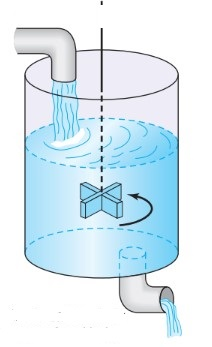
\includegraphics[scale=0.4]{Mezclas}  
                \caption{Sistema de Mezcla un tanque}
                \end{center}
                \end{figure}
                
            Utilizando este principio se dará solución al siguiente modelo.\cite{Zill2002d}
            \newpage
            
    
        \subsection{Problema}
        
            Se tiene una unidad de desinfección de agua la cual requiere del funcionamiento simultaneo de 2 tanques, uno donde se adicione el soluto (cloro granulado) y el otro que reciba el agua con solución. Ademas para un mejor mezclado se recomienda devolver al primer tanque una proporción de la solución recibida por el segundo tanque. Para que el proceso funcione correctamente y se pueda surtir a la toda la comunidad de manera continua, se requiere una capacidad por tanque de 500 galones y ademas se necesita conocer la concentración de cloro en los tanques en cualquier instante de tiempo t. \par
            Se describe el funcionamiento del sistema,
            
            \begin{figure}[ht]
                    \begin{center}
                    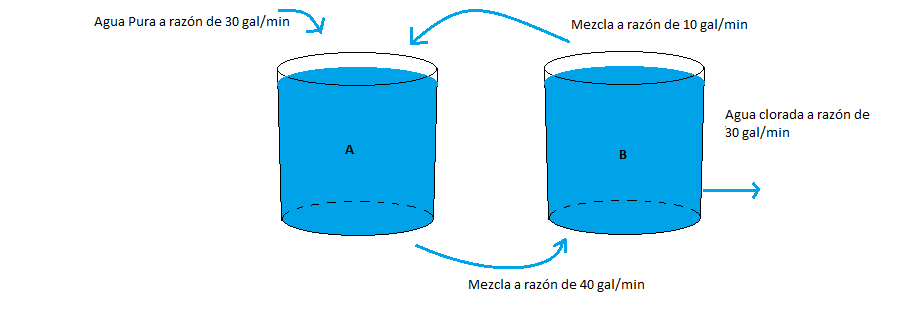
\includegraphics[scale=0.4]{SistemadeMezcla}  
                \caption{Sistema de Mezcla}
                \end{center}
            \end{figure}
            
            
            Se cuenta tambien con información al inicio del funcionamiento de la unidad.\vspace{0.1cm}
                
            La solución se desarrolla de la siguiente manera:\par\vspace{0.1cm}
            
            Siendo $X_1$ = Concentración de cloro en cualquier instante de tiempo t, en el tanque A, y siendo,\par\vspace{0.1cm}
            $X_2$ = Concentración de cloro en cualquier instante de tiempo t, en el tanque B.\vspace{0.1cm}
            
            Se conoce que al inicio del funcionamiento de la unidad, la concentración en el tanque A es 250 lb de Cloro granulado en solución, y en el tanque B es cero; esto es:
            
                \begin{equation*}
                    X_1(0) = 250
                \end{equation*}
            
                \begin{equation*}
                    X_2(0) = 0
                \end{equation*}
            
            Ahora, necesitamos encontrar una ecuación que describa la variacion de la concentración de cada tanque, entonces se plantea como estan variando las cantidades en los tanques de acuerdo a lo que entra y a lo que sale.\vspace{0.1cm}
            
            Para los tanques, se tiene que la variación de la concentración en cualquier instante t, está dada por la diferencia entre lo que entra y lo que sale, la concentración que entra y sale es función de la velocidad a la que esté entrando la solución y la concentración que esta posea por unidad de volumen. Tambien es importante y necesario mencionar que la razón de entrada y salida de los tanques es igual; basta con observar el esquema anterior y notar que las cantidades que entran en los tanques son iguales a las que salen de los mismos. Por tanto se considera que el volumen es constante y se asume que se trabajará a la máxima capacidad del tanque es decir 500 gal. Lo anterior se expresa de la siguiente manera:
            
                \begin{equation*}
                    X'_1(t) = (30\frac{gal}{min}*0\frac{lb}{gal} + 10\frac{gal}{min}*\frac{X_2}{500gal}) - 40\frac{gal}{min}*\frac{X_1}{500gal}
                \end{equation*}\vspace{0.1cm}
                
            Luego, realizando las operaciones se tiene:
                
                \begin{equation}
                    X'_1(t) = \frac{X_2}{50} - \frac{2X_1}{25}
                    \label{X1}
                \end{equation}\vspace{0.1cm}    
                
            Ahora, se realiza el mismo proceso para el segundo tanque.
            
                \begin{equation*}
                    X'_2(t)= 40\frac{gal}{min}*\frac{X_1}{500} - 10\frac{gal}{min}*\frac{X_2}{500gal} - 30\frac{gal}{min}*\frac{X_2}{500gal}
                \end{equation*}\vspace{0.1cm}
            
            Realizando las operaciones tenemos,
                
                \begin{equation}
                    X'_2(t) = \frac{2X_1}{25} - \frac{2X_2}{25}
                    \label{X2}
                \end{equation}\vspace{0.1cm}   
                
            A continuación se utilizará el método de determinantes para resolver el sistema formado por (\ref{X1}) y (\ref{X2}); reescribiendo tenemos,
            
                \begin{equation*}
                    DX_1 + \frac{2X_1}{25} - \frac{X_2}{50} = 0
                \end{equation*}
                \begin{equation*}
                    DX_2 + \frac{2X_2}{25} - \frac{2X_1}{25} = 0
                \end{equation*}
            
            Utilizando el metodo del operador diferencial, lo anterior se escribe como sigue, 
                
                \begin{equation*}
                    (D + \frac{2}{25})X_1 - \frac{X_2}{50} = 0
                \end{equation*}
                \begin{equation*}
                    (D + \frac{2}{25})X_2 - \frac{2X_1}{25} = 0
                \end{equation*}
            
            Ahora se encontrará el determinante y por la regla de Cramer podemos decir que,
            
                \begin{center}
                    $\begin{vmatrix}
                    
                        (D +  \frac {2}{25}) & \frac{-1}{50}\vspace{0.1cm} \\
                        \frac{-2}{25} & (D + \frac{2}{25})
                        
                    \end{vmatrix}\vspace{0.4cm}$
                    
                    
                \end{center}
                    \begin{equation}
                        = ((D + \frac{2}{25})^2 - \frac{1}{625})X_1 = 0
                        \label{5}
                    \end{equation}
                    
                Es igual a cero porque al aplicar el metodo de Cramer, se hace cero la columna de $X_1$ y al buscar determinante, éste será cero y por tanto queda un sistema homogeneo para $X_1$. Será igual para $X_2$.
                
                Desarrollando (\ref{5}) queda lo siguiente:
                
                    \begin{equation}
                        (625D^2 + 100D +3)X_1 = 0
                        \label{6}
                    \end{equation}\vspace{0.2cm}
                    
                Si se desarrolla para $X_2$ queda exactamente igual que (\ref{6}), es decir,
                
                    \begin{equation}
                        (625D^2 + 100D +3)X_2 = 0
                        \label{7}
                    \end{equation}\vspace{0.2cm}
                
                Resolviendo para encontrar raices queda así:
                    
                    \begin{equation*}
                        (625m^2 + 100m +3)X_2 = 0
                    \end{equation*}\vspace{0.2cm}
                    
                    \begin{equation*}
                        (25m + 3)(25m+1) = 0
                    \end{equation*}\vspace{0.2cm}
                    \begin{equation*}
                        m_1= \frac{-3}{25} ~~y~~ m_2=\frac{-1}{25}
                    \end{equation*}\vspace{0.2cm}
                    
                Como ya se tienen las raices, sabemos que la solución general de un sistema homogéneo, puede expresarse,
                    
                    \begin{center}
                        $X_1 = C_1e^{m_1t}$ $+~C_2e^{m_2t}$\par\vspace{0.2cm}
                        $X_1 = C_1e^{\frac{-3}{25}t}$ $+~C_2e^{\frac{-1}{25}t}$
    
                    \end{center}
                Sabemos que $X_2$ se resuelve de la misma manera entonces se tiene:
                    
                    \begin{center}
                        $X_2 = C_3e^{m_1t}$ $+~C_4e^{m_2t}$\par\vspace{0.2cm}
                        $X_2 = C_3e^{\frac{-3}{25}t}$ $+~C_4e^{\frac{-1}{25}t}$
    
                    \end{center}
                
                Ahora para poder encontrar las soluciones particulares del sistema, es decir libres de parámetros, se procedera a evaluar en (\ref{X1}) y (\ref{X2}) ya que las soluciones encontradas deben satisfacer las ecuaciones citadas anteriormente, y tambien se tendrá en cuenta las condiciones iniciales establecidas.\par
                
                Procedemos a derivar tanto $X_1$ como $X_2$ 
                    
                    \begin{equation*}
                        X_1' = -\frac{3}{25}C_1e^{\frac{-3}{25}t} -  \frac{1}{25}C_2e^{\frac{-1}{25}t}   
                    \end{equation*}
                    
                    \begin{equation*}
                        X_2' = -\frac{3}{25}C_3e^{\frac{-3}{25}t} - \frac{1}{25}C_4e^{\frac{-1}{25}t}   
                    \end{equation*}\vspace{0.2cm}
                    
                Si se reemplazan $X_1$,$X_2$,$X'_1$ y $X'_2$ en (\ref{X1}) y (\ref{X2}) respectivamente, se obtiene: 
            
                    \begin{equation*}
                        -\frac{3}{25}C_1e^{\frac{-3}{25}t} -  \frac{1}{25}C_2e^{\frac{-1}{25}t} = \frac{1}{50}C_3e^{\frac{-3}{25}t} + \frac{1}{50} C_4e^{\frac{-1}{25}t} - \frac{2}{25}C_1e^{\frac{-3}{25}t} - \frac{2}{25} C_2e^{\frac{-1}{25}t}
                    \end{equation*}
                
                Se sabe que todo sumando que tengan la forma $e^{\frac{-3}{25}t}$ por ejemplo, se pueden relacionar en una ecuación, de la siguiente manera
                
                    \begin{equation*}
                        -\frac{3}{25}C_1e^{\frac{-3}{25}t} = \frac{1}{50}C_3e^{\frac{-3}{25}t} - \frac{2}{25}C_1e^{\frac{-3}{25}t} 
                    \end{equation*}\vspace{0.2cm}
                Esto es, \vspace{0.2cm}
                    \begin{equation}
                        -\frac{3}{25}C_1 = \frac{1}{50}C_3 - \frac{2}{25}C_1 
                        \label{8}
                    \end{equation}\vspace{0.2cm}
                Para el sumando de la forma $e^{\frac{-1}{25}t}$, se tiene:
                
                    \begin{equation}
                        -\frac{1}{25}C_2 = \frac{1}{50}C_4 - \frac{2}{25}C_2 
                        \label{9}
                    \end{equation}
                Ya se tiene las ecuaciones que nos permitiran hallar dos coeficientes $C_i$ y dejar dos en términos de los dos otros dos coeficientes.
                    
                Resolviendo (\ref{8}) y (\ref{9}) respectivamente se tienen,\par
                
                Para $C_3$,
                
                    \begin{equation*}
                        -\frac{1}{25}C_1 = \frac{1}{50}C_3 
                    \end{equation*}\vspace{0.1cm}
                    \begin{equation*}
                        C_3 = -2C_1
                    \end{equation*}\vspace{0.2cm}
                Para $C_4$ se tiene, 
                    \begin{equation*}
                        \frac{1}{25}C_2 = \frac{1}{50}C_4 
                    \end{equation*}\vspace{0.1cm}
                    \begin{equation*}
                        C_4 = 2C_2
                    \end{equation*}\vspace{0.2cm}
                
                Habiendo encontrado relaciones entre los coeficientes que pertenecen a las soluciones del sistema, se procede a reescribir las soluciones, con estos valores de $C_3$ y $C_4$, y se tiene:
                
                    \begin{center}
                    
                        $X_1 = C_1e^{\frac{-3}{25}t}$ $+~C_2e^{\frac{-1}{25}t}$
    
                    \end{center}
                
                    \begin{center}
                    
                        $X_2 = -2C_1e^{\frac{-3}{25}t}$ $+~2C_2e^{\frac{-1}{25}t}$
    
                    \end{center}    
                Ahora bien, teniendo las dos ecuaciones en terminos de unicamente dos constantes ($C_1$ y $C_2$), ya se puede entrar a usar las condiciones iniciales del problema que se tenian ya que esta información permitirá su obtención.
                
                    \begin{equation*}
                        X_1(0) = 250
                    \end{equation*}
            
                    \begin{equation*}
                        X_2(0) = 0
                    \end{equation*}
                
                Evaluando las condiciones iniciales se tiene:
                
                    \begin{equation*}
                        C_1 + C_2 = 250
                    \end{equation*}    
                    
                    \begin{equation*}
                        -2C_1 + 2C_2 = 0
                    \end{equation*}\vspace{0.3cm}
                    
                Resolviendo para $C_1$ y $C_2$ se obtiene:
                    \begin{equation*}
                        C_1 = 125
                    \end{equation*}    
                    
                    \begin{equation*}
                        C_2 = 125
                    \end{equation*}
                Si reemplazamos los valores encontrados en las soluciones de $X_1$ y $X_2$ se obtienen las soluciones particulares del sistema para cualquier tiempo t, es decir:
                
                    \begin{center}
                    
                        $X_1 = 125e^{\frac{-3}{25}t}$ $+~125e^{\frac{-1}{25}t}$
    
                    \end{center}
                
                    \begin{center}
                    
                        $X_2 = -250e^{\frac{-3}{25}t}$ $+~250e^{\frac{-1}{25}t}$
    
                    \end{center}  
                    
    \section{Resultados}
    
        Habiendo obtenido el vector solución del sistema, es posible observar como varía la cantidad de cloro granulado en el agua con el paso de los minutos, mediante una gráfica generada por las funciones solución o componentes de dicho vector, ademas se adjuntan resultados de concentración para los primeros treinta minutos:
         
        
            
           
            
        Se puede observar como se van equilibrando las concentraciones de cloro en los tanques a lo largo del tiempo mientras se realiza la mezcla; un tanque pasa de tener agua pura es decir con concentración cero a una valor mayor de concentración, mientras que el otro tanque donde se dosificó, inicia con la cantidad necesaria de 250 lb.  
        
       
    \section{Conclusiones}
        
        \begin{itemize}
            \item Los sistemas de ecuaciones diferenciales lineales nos permiten modelar situaciones de la realidad a través de funciones que describen lo mejor posible, al fenómeno estudiado.
            
            \item Las ecuaciones diferenciales requieren un alto compromiso y para poder entenderlas se necesita de muchos conceptos que se enseñan previamente a este curso; de ahi la importancia de las ecuaciones diferenciales, ya que es una aplicación de los conceptos vistos en matemáticas generales, Calculo diferencial, integral y vectorial, ademas del algebra lineal que es una gran herramienta para la resolución de sistemas de Ecuaciones Diferenciales
            
            \item Mediante la física, las ecuaciones diferenciales se convierten en unas herramientas muy poderosas para la descripción de fenómenos cuyos parámetros se relacionan entre ellos.
            
        \end{itemize}
        
        \newpage
        
        
    \section{Anexos}  
        \subsection{Grafica y tabla de resultados}
        \begin{figure}[ht]
                    \begin{center}
                    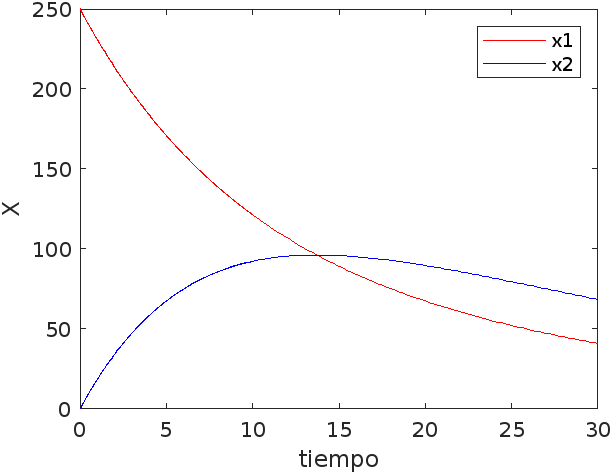
\includegraphics[scale=0.6]{Grafica30min} 
                \caption{Soluciones para t hasta treinta minutos.}
                \end{center}
                                        
                \begin{center}
                    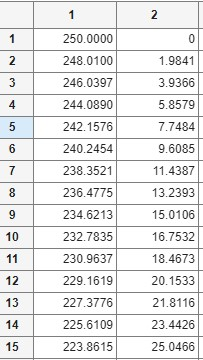
\includegraphics[scale=0.5]{Tabla1} 
                \caption{Resultados primeros quince minutos.}
                \end{center}
                
                \end{figure}
                
        \subsection{Código usado en Matlab}
			\subsubsection{Código para resolver sistema de ecuaciones diferenciales}            
            \begin{verbatim}
                % Universidad del Cauca
                % Ecuaciones Diferenciales
                % Solución de un sistema lineal de primer orden 2x2


                %Tiempo integración: Es el tiempo del intervalo en el que se dan las 
                %soluciones
                    ts = (0:0.2:30);

                %Condiciones Iniciales necesariar para la obtención de los coeficientes que
                %acompañan a las soluciones
                    x0 = [250,0];

                %Se resuelve mediante el solucionador ode45 función de Matlab para resolver
                %sistemas de ecuaciones diferenciales lineales:
                [t,x] = ode45(@SistemaEDLdePrimerOrden,ts,x0);

            %Esto se hace para la graficación de las soluciones del sistema; se ordena
            %la graficación de t y x ya sea X1 o X2. Los valores escritos como 'r' y
            %'b', son simplemente para darle el color a las grafica; hold on, significa
            %que se quiere que al graficar, se conserven las dos curvas.

                plot(t,x(:,1),'r'); hold on;

                plot(t,x(:,2),'b');

            % Etiquetas de los ejes coordenados

                legend('x1','x2'); xlabel('tiempo');

             ylabel('X');

            %Se introduce la variable del sistema, llamada dxdt; dxdt(1) y dxdt(2), son
            %las primeras derivadas de x(1) y x(2), como se puede observar en las
            %ecuaciones escritas, y estas son las ecuaciones obtenidas analiticamente,
            %observando el sistema interconectado de los tanques.

        function dxdt = SistemaEDLdePrimerOrden(t,x)

            dxdt(1) = (x(2)/50)-(2/25)*x(1);

            dxdt(2) = (2/25)*x(1) - (2/25)*x(2);

            dxdt = [dxdt(1);dxdt(2)];

                end    
            \end{verbatim}
        \subsubsection{Código para el calculo de determinantes de matrices cuadradas}    
        	\begin{verbatim}
        		%matriz a resolver (ejemplo)

A=[4 -5 2;1 -3 7;-2 6 4];

%Función que permite el calculo del determinante o Wroskiano de una matriz
function d=determinante(A)

		n=1:size(A,1);

		for k=1:size(A,1)

%La siguiente condición simplemente nos dice que si la matriz tiene un solo
%valor, es decir que sea 1x1, entonces el determinante es la misma matriz

    	if size(A,1)==1
        	d=A;
    	else
%Restricciones a tener en cuenta
        f=n(n~=1);
        
        c=n(n~=k);
%Se calcula determinante de K que va a variar y se suman los
%resultados:
        d(k)=((-1)^(1+k))*A(1,k)*determinante(A(f,c));
        
        d=sum(d);

%Para hallar determinante: en Command Window escribir det(A)
        
    end
end
end	
        	\end{verbatim}
                \newpage
                
    \begin{thebibliography}{15}
        
            \bibitem{Boyce2003}
            William E. Boyce and Richard E. DiPrima,
            \emph{Ecuaciones diferenciales y problemas con valores en la frontera},
            Pagina 353,
            Año 2003.
        
            \bibitem{Zill2002}
            Dennis G. Zill,
            \emph{Ecuaciones diferenciales con aplicaciones de modelado 7 ed.},
            Paginas 304-306,
            Año 2002.
            
            \bibitem{Kreyszing2003}
            Erwin Kreyszing,
            \emph{Matemáticas avanzadas para ingenieria},
            Paginas 195-196,
            Año 2003.
        
            \bibitem{Zill2002a}
            Dennis G. Zill,
            \emph{Ecuaciones diferenciales con aplicaciones de modelado 7 ed.},
            Paginas 306-308,
            Año 2002.
            
            \bibitem{Boyce2003a}
            William E. Boyce and Richard E. DiPrima,
            \emph{Ecuaciones diferenciales y problemas con valores en la frontera},
            Pagina 384,
            Año 2003.
            
            \bibitem{Zill2002b}
            Dennis G. Zill,
            \emph{Ecuaciones diferenciales con aplicaciones de modelado 9 ed.},
            Paginas 312-322,
            Año 2009.
            
            \bibitem{Zill2002d}
            Dennis G. Zill,
            \emph{Ecuaciones diferenciales con aplicaciones de modelado 7 ed.},
            Paginas 22-23,
            Año 2002.
            
        \end{thebibliography}
    
        
\end{document}